\subsection{Synthetic-control comparison}\label{app:scm}

Following \citet{abadie2010synthetic}, we construct a convex combination of
donor states using monthly counts of the Section~\ref{sec:prop19} family measure normalized by each state's
2018--2019 monthly mean. We choose weights to match the January 2018--May
2020 trajectory, ending the fitting window before the June 2020 ballot
announcement. The post-reform effect is the average proportional gap
relative to synthetic California in 2022--2023.
The comparison requires the weighted donor trajectory to approximate California's
untreated path beyond the fitting period. It does not net out market sales and
therefore targets a different comparison from the main triple difference.

The pre-period RMSPE is \PolicySCMFit\ percent. California's family-transfer
level is \PolicySCMDecline\ percent below synthetic California in 2022--2023.
The gap's interpretation depends on the quality of the donor trajectory
as a counterfactual, including California-specific shocks after May 2020.

\begin{figure}[!t]\centering
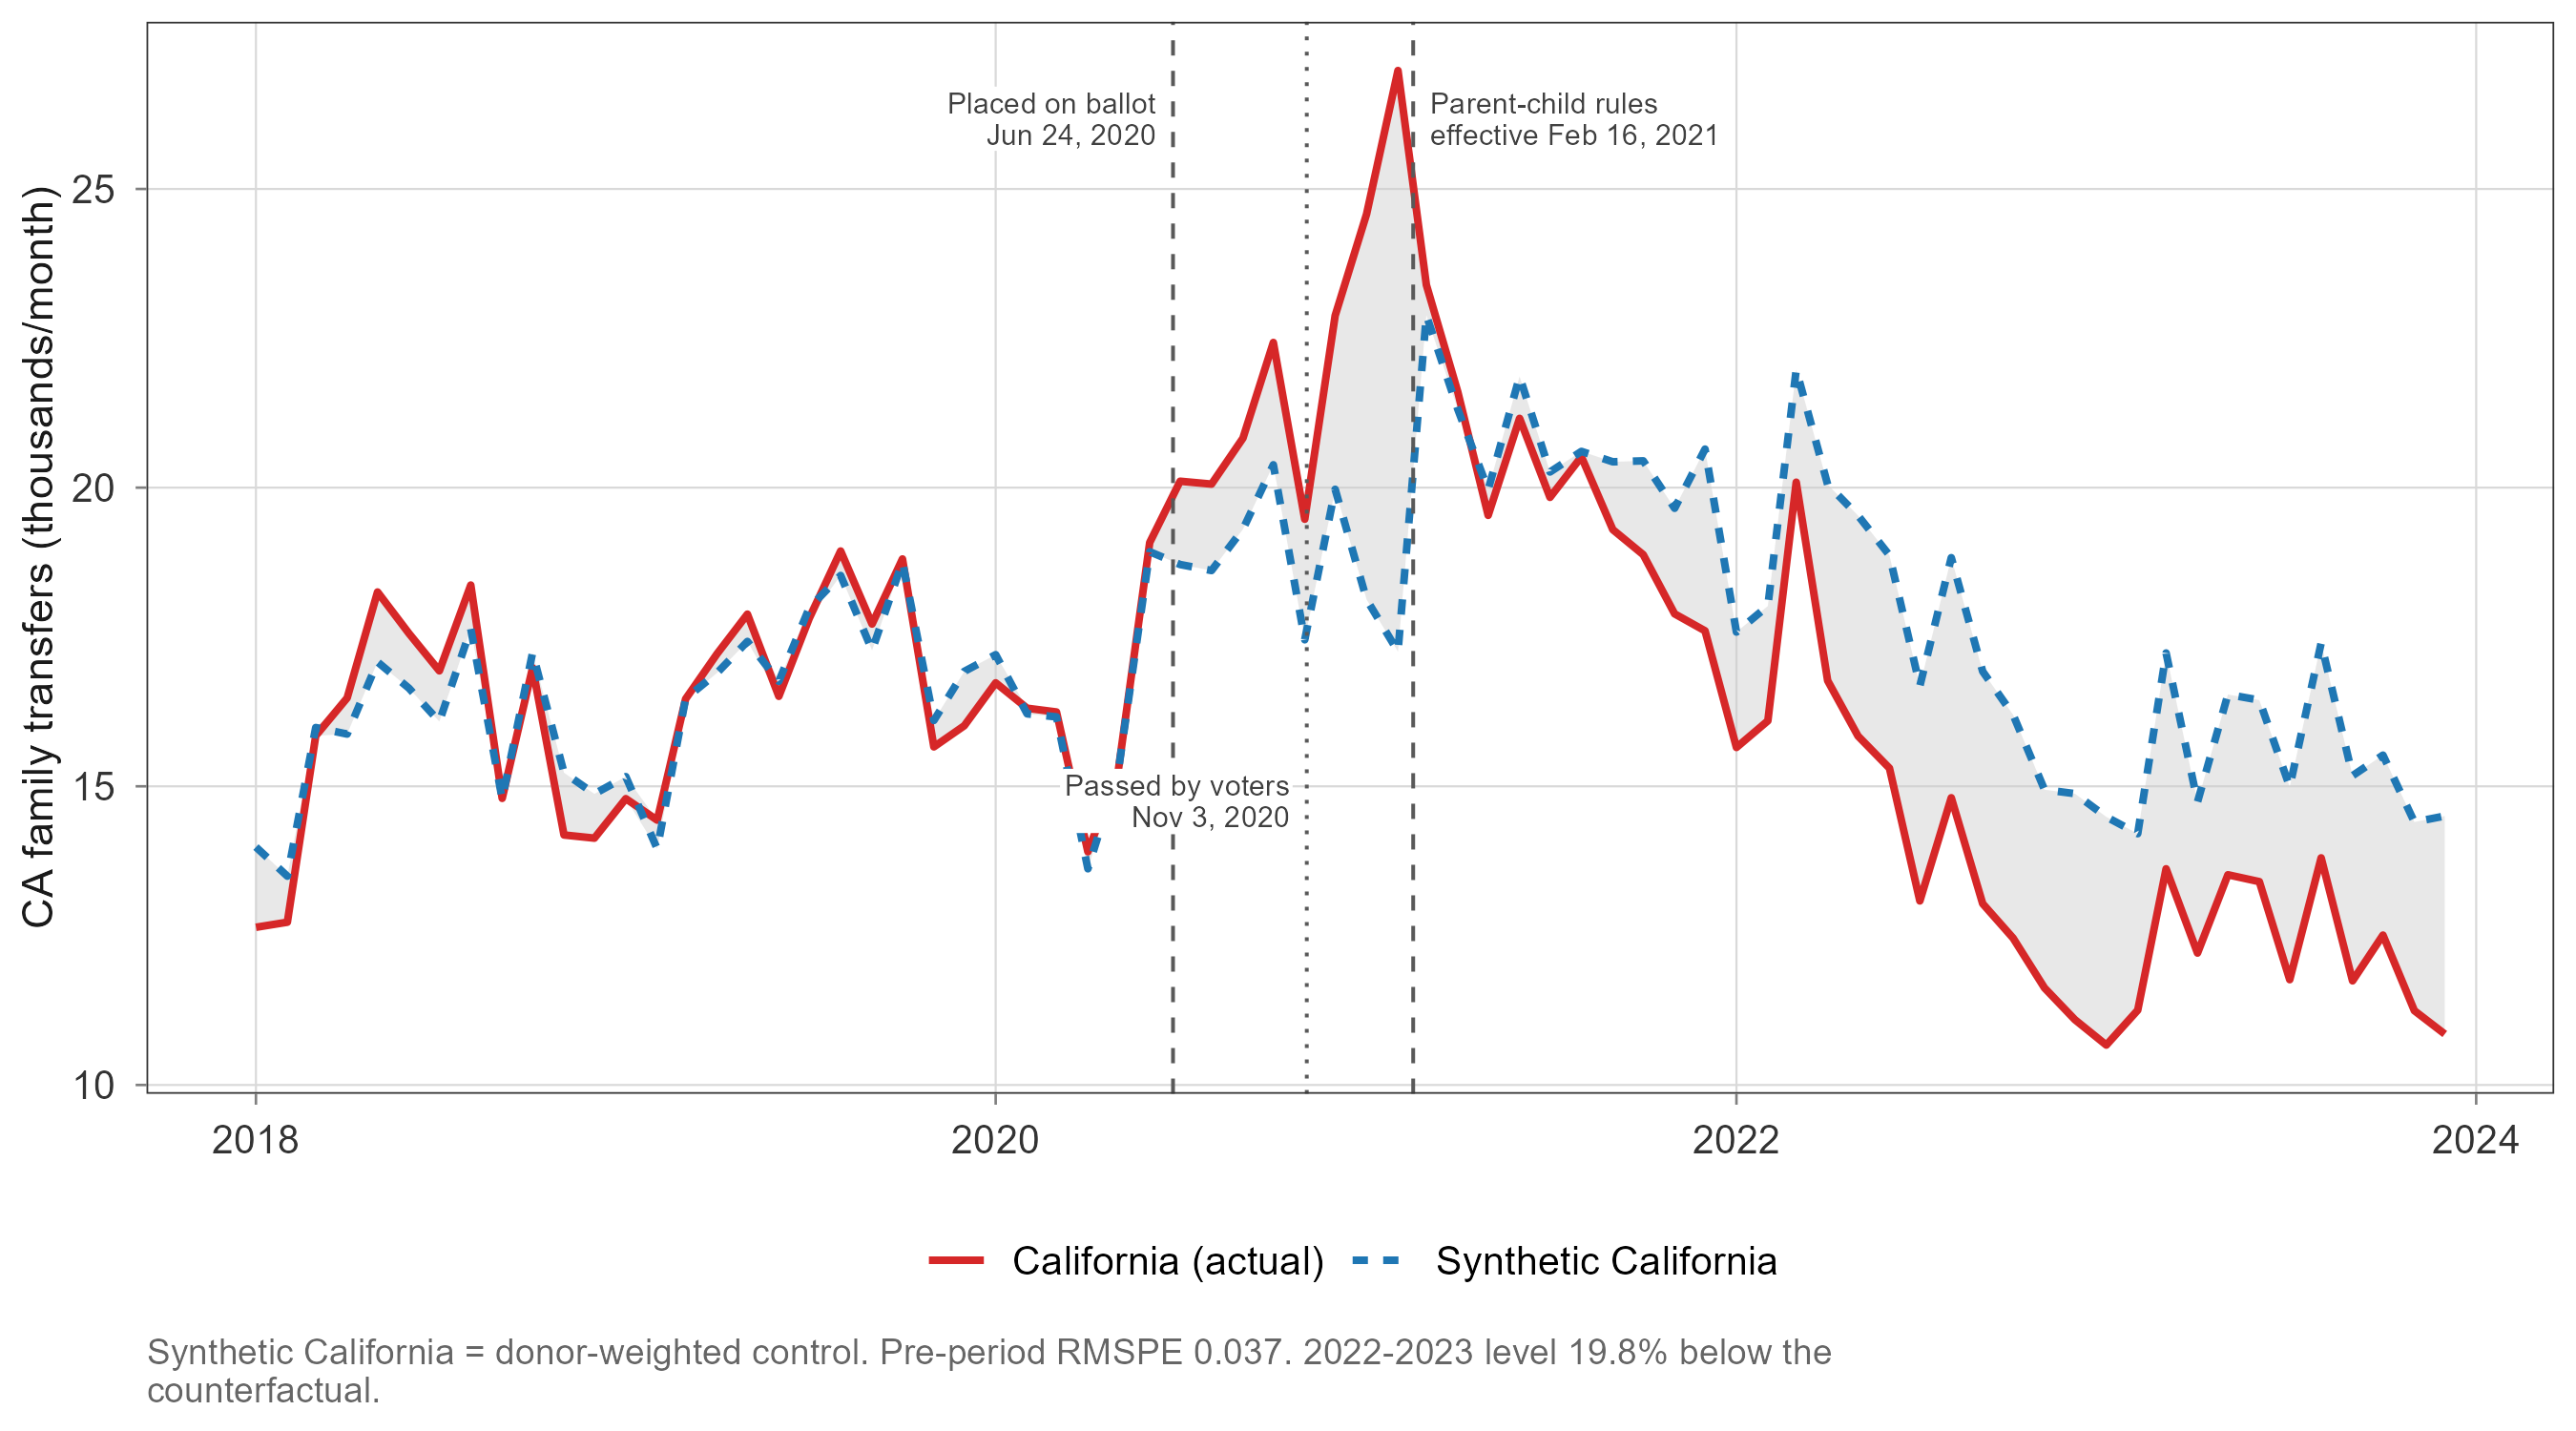
\includegraphics[width=0.9\linewidth]{figures/F5_scm_california.png}
\caption{California's family-transfer series, the Section~\ref{sec:prop19} measure of distinct people without affidavits of death and with chain-verified trust-to-heir deeds, and a donor-weighted synthetic California, normalized by each state's 2018--2019 monthly mean. Weights fit January 2018--May 2020.}\label{fig:scm}
\end{figure}


\paragraph{Demographic adjustment.} Re-estimating the synthetic control on
family transfers per resident aged 65 and over uses the same fitting window
and policy timing, with American Community Survey one-year population estimates
and interpolated 2020 population. Its pre-period RMSPE is \PolicySCMPCFit\ percent
and the 2022--2023 gap is \PolicySCMPCDecline\ percent below its counterfactual.
The two SCM estimates use different denominators and do not form a confidence interval.
